%%
%% This is file `sample-sigconf.tex',
%% generated with the docstrip utility.
%%
%% The original source files were:
%%%%
%% This is file `sample-sigconf.tex',
%% generated with the docstrip utility.
%%
%% The original source files were:
%%
%% samples.dtx  (with options: `sigconf')
%% 
%% IMPORTANT NOTICE:
%% 
%% For the copyright see the source file.
%% 
%% Any modified versions of this file must be renamed
%% with new filenames distinct from sample-sigconf.tex.
%% 
%% For distribution of the original source see the terms
%% for copying and modification in the file samples.dtx.
%% 
%% This generated file may be distributed as long as the
%% original source files, as listed above, are part of the
%% same distribution. (The sources need not necessarily be
%% in the same archive or directory.)
%%
%% The first command in your LaTeX source must be the \documentclass command.
\documentclass[sigconf]{acmart}


\settopmatter{printacmref=false} % Removes citation information below abstract
\renewcommand\footnotetextcopyrightpermission[1]{} % removes footnote with conference information in first column
\pagestyle{plain} % removes running headers

%%
%% custom packages
\usepackage[utf8]{inputenc}
\usepackage{booktabs}
\usepackage{tabularx}
\usepackage{booktabs}
\usepackage[autostyle=true]{csquotes}
\usepackage{xpatch}
\usepackage{graphicx}  %%% for including graphics
\graphicspath{{./images/}}
\usepackage{url}       %%% for including URLs
\usepackage{times}
\usepackage{amsmath}
\usepackage{float}
%caption size
\usepackage{caption}
\captionsetup[figure]{font=small,labelfont=small}
\captionsetup[table]{font=small,labelfont=small}


%Conference
\acmConference[CS7IS3]{INFORMATION RETRIEVAL AND WEB SEARCH}{April 2020}{Trinity College Dublin, Ireland} 
\acmYear{2020}
\copyrightyear{2020}
\acmPrice{00.00}

%%
%% \BibTeX command to typeset BibTeX logo in the docs
\AtBeginDocument{%
  \providecommand\BibTeX{{%
    \normalfont B\kern-0.5em{\scshape i\kern-0.25em b}\kern-0.8em\TeX}}}

%% Rights management information.  This information is sent to you
%% when you complete the rights form.  These commands have SAMPLE
%% values in them; it is your responsibility as an author to replace
%% the commands and values with those provided to you when you
%% complete the rights form.


%% These commands are for a PROCEEDINGS abstract or paper.



%%
%% Submission ID.
%% Use this when submitting an article to a sponsored event. You'll
%% receive a unique submission ID from the organizers
%% of the event, and this ID should be used as the parameter to this command.
%%\acmSubmissionID{123-A56-BU3}

%%
%% The majority of ACM publications use numbered citations and
%% references.  The command \citestyle{authoryear} switches to the
%% "author year" style.
%%
%% If you are preparing content for an event
%% sponsored by ACM SIGGRAPH, you must use the "author year" style of
%% citations and references.
%% Uncommenting
%% the next command will enable that style.
%%\citestyle{acmauthoryear}

%%
%% end of the preamble, start of the body of the document source.
\begin{document}

%%
%% The "title" command has an optional parameter,
%% allowing the author to define a "short title" to be used in page headers.
\title{Information Retrieval Group Report\\Group 4 - InfoSeekers}

%%
%% The "author" command and its associated commands are used to define
%% the authors and their affiliations.
%% Of note is the shared affiliation of the first two authors, and the
%% "authornote" and "authornotemark" commands
%% used to denote shared contribution to the research.
\author{Ashwin Sundareswaran R}
\email{ramasuba@tcd.ie}
\affiliation{%
  \institution{Trinity College Dublin}
  \streetaddress{College Green}
  \city{Dublin 2}
}

\author{Chao Chen}
\email{chenc1@tcd.ie}
\affiliation{%
  \institution{Trinity College Dublin}
  \streetaddress{College Green}
  \city{Dublin 2}
}

\author{Chia Lau}
\email{LAUCH@tcd.ie}
\affiliation{%
  \institution{Trinity College Dublin}
  \streetaddress{College Green}
  \city{Dublin 2}
}

\author{Vishal Kumar}
\email{kumarv1@tcd.ie}
\affiliation{%
 \institution{Trinity College Dublin}
 \streetaddress{College Green}
 \city{Dublin 2}
}

%%
%% By default, the full list of authors will be used in the page
%% headers. Often, this list is too long, and will overlap
%% other information printed in the page headers. This command allows
%% the author to define a more concise list
%% of authors' names for this purpose.
\renewcommand{\shortauthors}{Group 4 - InfoSeekers}

%%
%% The abstract is a short summary of the work to be presented in the
%% article.
\begin{abstract}
  Information retrieval is an important concept in today’s information world. An efficient search engine helps users to obtain the relevant information even if the query is not properly framed. Lucene is one such library in Java used to index and search the dataset provided as input to it. It has an in-built analyzers object used to index the words and rank it accordingly. Data from four different sources including Financial Times Limited, Federal Register, Foreign Broadcast Information Service, Los Angeles Times were the input corpora for the query to be processed. A separate topic file is selected as a query file and the result of 1000 hits per topic is considered for evaluation. Custom analyzers based on synonyms are built to analyze the indexed data and to query.
\end{abstract}

%%
%% The code below is generated by the tool at http://dl.acm.org/ccs.cfm.
%% Please copy and paste the code instead of the example below.
%%

%%
%% Keywords. The author(s) should pick words that accurately describe
%% the work being presented. Separate the keywords with commas.
\keywords{Information Retrieval, Search Engine, Analyzers, Scorers, Lucene, Synonym}

%% A "teaser" image appears between the author and affiliation
%% information and the body of the document, and typically spans the
%% page.

%%
%% This command processes the author and affiliation and title
%% information and builds the first part of the formatted document.

\maketitle
\vspace{2mm}
\section{Introduction}
Information Retrieval is the process of finding the relevant information in a document and presenting the result when a query is made.
Lucene\cite{lucene} is a library built in java made specifically to implement search engines and provide relevant information to users.
Data considered for the process of finding the relevance is the collection of different articles from four different news publishers including Financial times limited, Federal Register, Foreign Broadcast Information Service and Los Angeles Times.
There are articles from various domains including medicine, philosophy, economics, tourism etc and each of the publisher has more than 10 documents containing articles in each of them.
The articles are published and maintained by National Institute of Standards and Technology(NIST) to make it available for the research community to work on improving the techniques for handling the information retrieval process.
The data in the corpora is in the form of Standard Generalized Markup Language(SGML) and this is parsed using Jsoup\cite{jsoup}, a library used to parse HTML and URL.Each field in the article is parsed in separate index and the same is stored for analyzing with the provided query.
A query file is provided and the same is parsed to obtain the separate fields from it which is then queried along the indexed data corpora.A custom analyzer is built which is used to analyze the indexed documents with respect to the provided query.
The analyzer is built in which custom stop words were made to be removed from the document while querying the same.This list of stop words is chosen based on the trial performed on the process of evaluating with Trec\_Eval\cite{trec_eval}, and the top list is selected which provides the maximum relevancy result.
Trec\_Eval is maintained by National Institute of Standards and Technology which release the evaluation files  which is considered as gold standard for comparing the performance of the obtained result.
Moving average precision score is calculated and the goal is to improve the score so that the performance of the search engine is also optimised.
\vspace{0.2cm}
\section{Pre-processing on Corpora}

We tried to pre-process the corpora (mainly the given corpora from newspapers) with 2 ways.
The corpora are first renamed with suffixes \enquote{*.sgm} and the folder structure is re-organized for file filtering purpose.

\subsection{SGML to JSON}

The tool \enquote{osx} from OpenSP\cite{openSP} is an SGML tool converting documents from SGML to XML. The tool, \enquote{osx}, can read the \enquote{*.dtd} files for structure definitions of the file. After getting parsed XML files, we use the script \enquote{hay/xml2json} to parse files from XML to JSON. The reason we want JSON files is that the structures of JSON files are closer to the structures of objects in Java.

But the process produced many useless fields in the parsed files, we finally drop this solution.

\subsection{Jsoup}

Jsoup is a library for processing HTML or other SGML-like standard language written in Java. Elements of the SGML files are identified and texts inside the element can be extracted. For the 4 types of documents, the program parses with these elements identified:
\vspace{.1cm}
\begin{itemize}
    \item \textbf{Foreign Broadcast Information Service(FBIS):} DOCNO, TEXT, PROFILE, DATE, HEADLINE, BYLINE, PUB, PAGE.
    \item \textbf{Federal Register(FR94):} DOCNO, TEXT, META, PARENT, HEADLINE.
    \item \textbf{Financial Times Limited(FT):} DOCNO, TEXT, PROFILE, DATE, HEADLINE, BYLINE, PUB, PAGE.
    \item \textbf{Los Angeles Times(LATIMES):} DOCNO, TEXT, DOCID, DATE, SECTION, LENGTH, HEADLINE, GRAPHIC, TYPE, SUBJECT, BYLINE.
\end{itemize}

To notice that in case of some elements might be ignored, we pick the texts off from the document one by one and the rest of the content goes into an extra element called \enquote{META}.

\subsection{Jsoup Query Parsing}

A custom query parser is built using Jsoup library in Java to parse the topic file which has 50 query present in it. The various fields from the query files are parsed and stored separately for analyzing the index files. The different content are present in the query file are parsed into separate fields NUM, TITLE, DESCRIPTION, NARRATIVE and converted into lower case letters to make it all uniform in case.
\vspace{0.2cm}



\section{Analyzers}

In order to index different words of the dataset provided, the important terms need to be picked. This is done by stemming various words into tokens and removing the various stop words and then finding in which documents the tokenized terms are present. Lucene has a separate library comprising the analyzers which performs tokenization operation in the input dataset provided to it. The following different analyzers performs the operation in different ways as follows:

\subsection{Standard Analyzer}

This is a basic analyzer that is capable of handling names, e-mail address etc. It lowercases all the words and then tokenizes them. It also removes common words and punctuation.

\subsection{English Analyzer}

This analyzer is specially built for supporting English language. It uses special filter like English Possessive Filter, Keyword maker filter which makes it powerful compared to other analyzers in tokenizing words in English language.

\subsection{Analyzer using ShingleFilter}

One Lucene filter which looked promising was the Shingle Filter. Given a stream of tokens, e.g.: “To be or not to be”. It would output shingles: “To be”, “be or”, “or not”, “not to”, “to be”.

Arguments to this filter would dictate how many tokens per shingle and if the original tokens (“to”, “be”, etc) would be included in the output.

This sounded promising as the dataset contained queries looking for certain two word combinations. For example, Query 421 looks for “industrial waste” as opposed to “radioactive waste” or “dumping waste”.

Unfortunately, this seems to be a dead end. It would take much more time and memory to index. Furthermore, it did not ultimately help increase the Mean Average Precision(MAP).

\subsection{Custom Analyzers}

Customized analyzers are introduced in this section.

\subsubsection{Customized Analyzer}\hfill
\newline
The first customized analyzer (CUSTOM1) is described below.

The processing of the text starts with a StandardTokenizer and then goes through a stack of filters:

\begin{itemize}
    \item LowerCaseFilter: to lower the cases.
    \item TrimFilter: to trim whitespace characters.
    \item EnglishPossessiveFilter: to get rid of possessives (e.g. “it's” to “it”).
    \item SetKeywordMarkerFilter: to skip the words with a list provided. We define the list manually when going through the queries.
    \item EnglishMinimalStemFilter: to transform plurals into singulars.
    \item StopFilter: to remove words with a list of stopwords provided.
    \item PorterStemFilter: a stemming algorithem provided by Snowball scripts\cite{porterStemmer}.
\end{itemize}

\subsubsection{Customized Analyzer with Synonyms}\hfill
\newline
Based on CUSTOM1, we introduced a new customized analyzer with Synonyms (CUSTOM2). A SynonymTokenFilter is added just before the PorterStemFilter. The SynonymTokenFilter implements a function to generate synonyms from a SynonymMap. The SynonymMap can be considered as a lexicon, we parsed the SynonymMap from a file called “wn\_s.pl” from WordNet\cite{wordnet}. The WordNet version is 2.1 and the file is written in Prolog, containing synonym pairs information. Then the queries are expanded by searching both original texts and their synonyms, and the max count of synonyms from a word is set to 3 in our implementation.

\subsubsection{Graph Filter based Custom Analyzer}\hfill
\newline
In progression to customise analyser, we added another analyzer as “CustomAnalyzer\_Syn\_stp” referred as "CUSTOM3" in code. It includes StandardTokenizer\cite{StandardTokenizer} as  main tokeniser, Classic Token Stream and some token filter as Snowball\cite{snowball_filter} stemming algorithm, stop word filter for most commonly used words, and synonym graph filter for country names with word delimiter filter to split words into sub-words to make efficient token graph.



\section{Scoring Models}

Searcher performs query search in the indexer and provides the top 1000 hits of the search result. It is the work of the scorer to provide relevance score for the queried results which we have obtained and marks a score which signifies the click through rate of the user in terms of real search engine. There are various methods to calculate this score and the following were tested:

\subsection{TF-IDF (Classic Similarity)}

This uses the vector space model to calculate the term frequency and then calculate how important that term is in the document retrieved and based on that the score is provided for the texts. For example, the commonly occurring words (ex: the, a) receive very less score in considering complex terms like “judicial”.

\subsection{BM25 Similarity}

This is similar in methodology while comparing with the TF-IDF but since TF-IDF can produce negative scores for the term based on the frequency, this has rectified it by adding a 1 on top of log such that only positive values of the scores is obtained and thus having an equal scale for all the scores making it more reliable.

\subsection{Boolean Similarity}

This is a classic Boolean scorer which provides a positive score if all the terms or selected terms are present in the retrieved file. This is useful in searches where we want both the search terms to be present in the queried document.

\subsection{LMDirichlet Similarity}

This similarity is introduced to have better performance in comparing the documents and getting better results.The formula for this assigns a negative score to documents that contain the term, but with fewer occurrences than predicted by the other scorers and increasing the scoring evaluation.

\subsection{LMJelinekMercer Simialrity}

This similarity is working by including a parameter which can be varied, so as to include the required percentage of query words in the result. This parameter needs to be selected correctly to make the scorer work fine and produce better performance.
 
 \vspace{.5cm}


\section{Results and Evaluation}

The queries are passed to a MultiFieldQueryParser, with searching fields boost:

\begin{itemize}
    \item HEADLINE: 0.1
    \item TEXT: 0.9
\end{itemize}
\vspace{.07cm}
In Table \ref{tab:maps}, MAP results are mentioned for set of different scoring models and analyzers included in code.
\begin{table}[!htbp]
  \caption{Mean Avrage Precision(MAP) from the experiments}
  \label{tab:maps}
  \centering
  \renewcommand{\tabularxcolumn}{m} % we want center vertical alignment
  \begin{tabularx}{0.8\linewidth}{l | l | l}
    \toprule
    Scoring         & Analyzer & MAP$\times 10^{-4}$
    \tabularnewline \hline
    BM25            & Standard & 2483
    \tabularnewline \hline
    BM25            & English  & 3115
    \tabularnewline \hline
    BM25            & CUSTOM1  & 3147
    \tabularnewline \hline
    BM25            & CUSTOM2  & 2697
    \tabularnewline \hline
    BM25            & CUSTOM3  & 3200 *
    \tabularnewline \hline
    Classic         & CUSTOM3  & 1783
    \tabularnewline \hline
    LMDirichlet     & CUSTOM3  & 2896
    \tabularnewline \hline
    LMJelinekMercer & CUSTOM3  & 3245 *
    \tabularnewline \bottomrule
  \end{tabularx}
\end{table}
\newline
The best combination is the LMJelinekMercer scorer with CUSTOM3 analyzer(MAP=0.3245), and a 2nd choice which is BM25 with CUSTOM3 analyzer(MAP=0.3200).
\newline
\\
Graphs are generated for these set of scoring and analyzer models. Gnuplot\cite{gnuplot} library is used with precision-recall and precision-document count data from trec eval\cite{trec_eval} result.
In figure \ref{fig:exp1} and \ref{fig:exp2} comparison curve is shown for different analyzers and with BM25 scoring model. In Figure \ref{fig:exp3} and \ref{fig:exp4} different similarity models  are compared with CUSTOM3 analyzer.
\vspace{15mm}
\newline
\begin{figure}[!htbp]
  \centerline{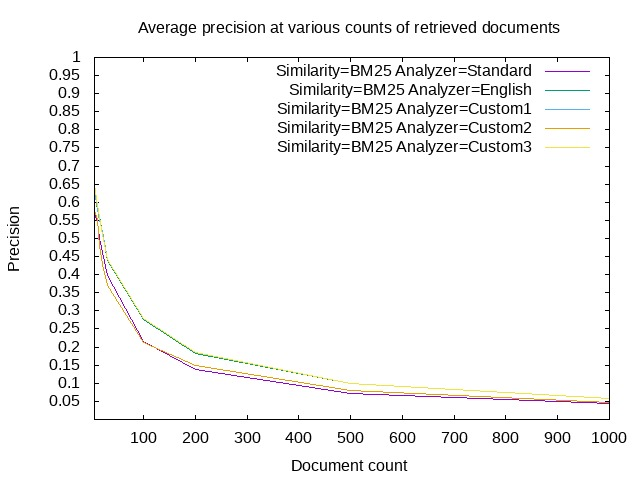
\includegraphics[width=8cm, height=6cm]{images/avg_pre_bm25.jpg}}
  \vspace*{-3mm}
  \caption{Average precision at different number of retrieved documents using BM25 Similarity}
  \label{fig:exp1}
\end{figure}
\vspace*{-4mm}
\begin{figure}[!htbp]
  \centerline{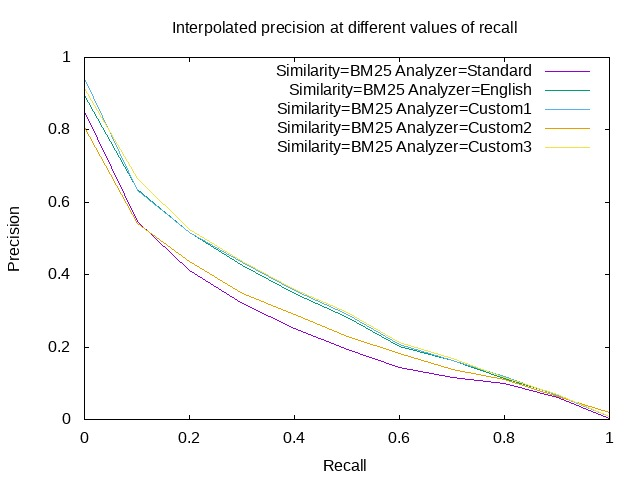
\includegraphics[width=8cm, height=6cm]{images/pr_bm25.jpg}}
  \vspace*{-3mm}
  \caption{Interpolated precision at different values of recall using BM25 Similarity}
  \label{fig:exp2}
\end{figure}
\vspace*{-4mm}
\begin{figure}[!htbp]
  \centerline{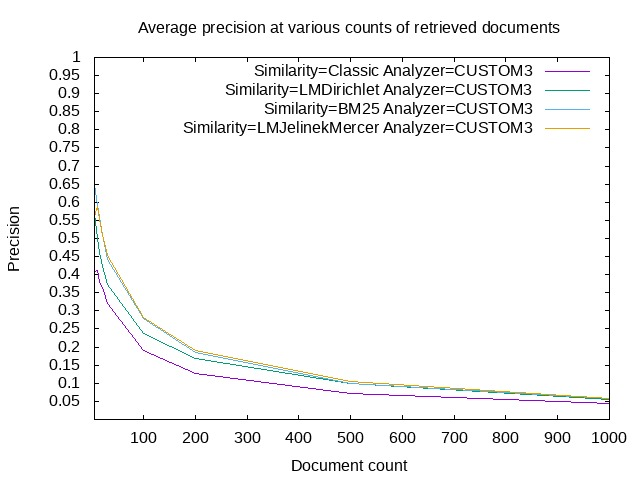
\includegraphics[width=8cm, height=6cm]{images/avg_pre_cus3.jpg}}
  \vspace*{-3mm}
  \caption{Average precision at different number of retrieved documents using CUSTOM3 analyzer with various Similarities}
  \label{fig:exp3}
\end{figure}
\vspace*{-4mm}
\begin{figure}[!htbp]
  \centering
  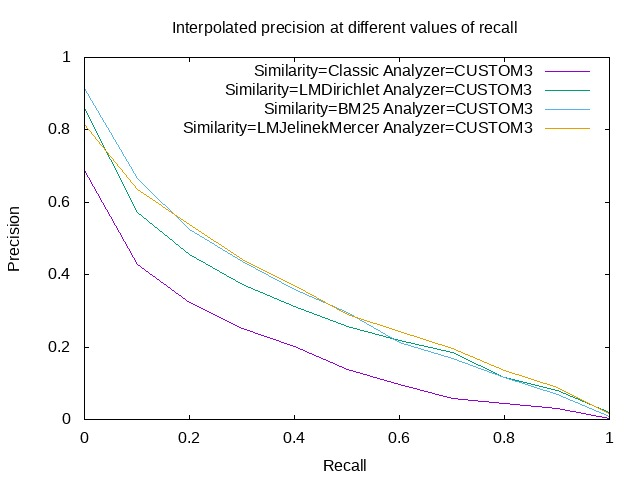
\includegraphics[width=\linewidth]{images/pr_cus3.jpg}
  \vspace*{-3mm}
  \caption{Interpolated precision at different values of recall using CUSTOM3 analyzer with various Similarities}
  \label{fig:exp4}
\end{figure}

\section{Summary}

In this work we did a comparison on the existing analyzers and scorers provided by Lucene. A group of cuntomized analyzers are implemented with refined word lists, like longer stopwords list and special terms and words like countries. We also make use of synonym query expanding and graph query. We find that the hyperparameters (boosts) of the query parser affect the result critically, and we believe other hyperparameters for the analyzers are also important. A broader research should be made on the processing and a better way is needed for cross validation.
\vspace{2mm}


%%
%% The next two lines define the bibliography style to be used, and
%% the bibliography file.
\bibliographystyle{ACM-Reference-Format}
\bibliography{bibfile}

%%
%% If your work has an appendix, this is the place to put it.
\vspace{2cm}
\appendix
\section{APPENDIX}
\subsection{Instructions}

This section contains the instruction to access the instance, with information about this project (the journal and the repository).

A user called \enquote{ubuntu} comes with sudo permissions:

\begin{itemize}
    \item username: ubuntu
    \item ip: 54.235.6.210
    \item port: 22
    \item password: HXfEmkrh
\end{itemize}

The project is present at the home folder of the user.

Please see \enquote{README.md} file for more instructions on running the program.

Also there are prepared result files:

\begin{itemize}
    \item result\_phaseII\_LMJelinekMercer\_Custom3
    \item result\_phaseII\_BM25\_Custom3
\end{itemize}

in the project root folder for the final judgement.
\vspace{2mm}
\newline
The journal can be accessed via a \enquote{tcd.ie} email account:

\url{https://docs.google.com/document/d/1xdgEgsakmC1qhJoqi014SGc0_mka-OtL30ERPGPUs1s/edit#}
\vspace{2mm}
\newline
The repository will be public after the submission:

\url{https://github.com/tannineo/cs7is3-team4}



\end{document}
\endinput
%%
%% End of file